\chapter{はじめに}
\section{宇宙での元素合成過程}
\label{seq::nucleaosynthesis}
身の回りには多種多様な物質が存在している。
これらの物質は原子が組み合わさることで形成される。
現在の地球には水素 (原子番号1) からウラン (原子番号92) までの元素が天然で存在してる。
原子は更に小さい原子核と電子で構成されており、原子核は陽子と中性子で構成されている。
現在までに天然、人工合わせて118種類の元素が確認されている。
しかし、ビッグバン直後には水素とヘリウムと僅かな軽元素しか存在していなかった。
これは、A (質量数) が5及び8の安定な原子核が存在しないことに由来する。
ヘリウム ($\alpha$) は安定な原子核である。
2つの$\alpha$が反応に${}^{8}\rm{He}$が生成されるが、
2つの$\alpha$に分裂するほうが安定であるためすぐに崩壊してしまう。
同様にA = 5の原子核が生成してもすぐに軽い核2つに分裂してしまう。

宇宙初期では水素を主成分とする恒星しか存在しなかったと考えられる。
このような恒星が重力により収縮し中心温度が$10^7~\rm{K}$を超えると、
ppチェインによって水素の燃焼が行われるようになる。
ppチェインでは式 (\ref{eq::pp1}) (\ref{eq::pp2}) (\ref{eq::pp3})に示した3つの系列が重要とされる。
どの系列も最終的には4つの陽子から1つの$\alpha$粒子を生成している。
%\begin{gather}
%  \rm{p}(\rm{p},\beta^{+}\nu)\rm{d}(\rm{p},\gamma){}^{3}\rm{He}({}^{3}\rm{He},2\rm{p})\alpha\label{eq::pp1}\\
%  \rm{p}(\rm{p},\beta^{+}\nu)\rm{d}(\rm{p},\gamma){}^{3}\rm{He}(\alpha,\gamma){}^{7}\rm{Be}(\rm{e}^{-},\nu){}^{7}\rm{Li}(\rm{p},\alpha)\alpha\label{eq::pp2}\\
%  \rm{p}(\rm{p},\beta^{+}\nu)\rm{d}(\rm{p},\gamma){}^{3}\rm{He}(\alpha,\gamma){}^{7}\rm{Be}(\rm{p},\gamma){}^{8}\rm{B}(\beta^{+}\nu){}^{8}\rm{Be}(\alpha)\alpha\label{eq::pp3}
%\end{gather}
\begin{gather}
  \begin{array}{llll}
    \rm{p} + \rm{p} \rightarrow & \rm{d} + \beta^{+} + \nu & &\\
    & \rm{d} + \rm{p} \rightarrow & {}^{3}\rm{He} + \gamma &\\
    & & {}^{3}\rm{He} + {}^{3}\rm{He} \rightarrow & \alpha +2\rm{p}
  \end{array}\label{eq::pp1}\\  
  \begin{array}{llllll}
    \rm{p} + \rm{p} \rightarrow & \rm{d} + \beta^{+} +\nu & & & &\\
    & \rm{d} + \rm{p} \rightarrow & {}^{3}\rm{He} + \gamma & & &\\
    & & {}^{3}\rm{He} + \alpha \rightarrow & {}^{7}\rm{Be} & &\\
    & & & {}^{7}\rm{Be} + \rm{e}^{-} \rightarrow & {}^{8}\rm{Li} + \nu &\\
    & & & & {}^{7}\rm{Li} + \rm{p} \rightarrow & \alpha + \alpha
  \end{array}\label{eq::pp2}\\
  \begin{array}{lllllll}
    \rm{p} + \rm{p} \rightarrow & \rm{d} + \beta^{+} + \nu & & & & &\\
    & \rm{d} + \rm{p} \rightarrow & {}^{3}\rm{He} + \gamma & & & &\\
    & & {}^{3}\rm{He} + \alpha \rightarrow & {}^{7}\rm{Be} + \gamma & & &\\
    & & & {}^{7}\rm{Be} + \rm{p} \rightarrow & {}^{8}\rm{B} + \gamma & &\\
    & & & & {}^{8}\rm{B} \rightarrow & {}^{8}\rm{Be} + \beta^{+} + \nu &\\
    & & & & & {}^{8}\rm{Be} \rightarrow & 3\alpha
  \end{array}\label{eq::pp3}
\end{gather}

ppチェインにより水素燃焼が十分に行われた恒星では水素よりも重いヘリウムが
より恒星の中心に集まりヘリウムの核 ($\rm{He}$コア) を生成する。
$\rm{He}$コアが重力により圧縮され温度がおよそ$10^8~\rm{K}$に達するとヘリウム燃焼が始まる。
$\rm{He}$コアには十分な量の$\alpha$が存在するため、2つの$\alpha$が融合し${}^{8}\rm{Be}$となる。
恒星中では${}^{8}\rm{Be}$が崩壊するより早くもう1つ$\alpha$が融合して${}^{12}\rm{C}^{*}$になる。
このときに作られる${}^{12}\rm{C}$の励起状態はFred Hoyle が予言した$3\alpha$の
共鳴状態 (Hoyle状態、$\rm{Ex} = 7.65\rm{MeV}$、$0_{2}^{+}$) である。
Hoyle状態の${}^{12}\rm{C}$が脱励起し基底状態 (g.s.) になる (式(\ref{eq::triplealpha})) 。
この3つの$\alpha$粒子が融合し${}^{12}\rm{C}$が生成される反応はトリプルアルファ反応と呼ばれる。
トリプルアルファ反応が恒星中で起こることでA = 5, 8の壁を乗り越えることができる。
生成された${}^{12}\rm{C}$が更に$\alpha$を吸収することで$\rm{O}$や$\rm{Si}$などの更に重い核の合成へ進んでいく。
\begin{equation}
  \begin{array}{llll}
%  \alpha(\alpha,\gamma){}^{8}\rm{Be}(\alpha,{}^{12}\rm{C}^{Hoyle})
%  \alpha(\alpha,\gamma){}^{8}\rm{Be}+\alpha\rightarrow{}^{12}\rm{C}^{Hoyle}\label{eq::triplealpha}
  %あとで矢印の絵を書こうかな
    \alpha + \alpha \rightarrow & {}^{8}\rm{Be} & & \\
    & {}^{8}\rm{Be} + \alpha \rightarrow & {}^{12}\rm{C}^{Hoyle} &\\
    & & {}^{12}\rm{C}^{Hoyle} \rightarrow & {}^{12}\rm{C} + \gamma
  \end{array}\label{eq::triplealpha}
\end{equation}

\section{高温高密度中でのトリプルアルファ反応}
\label{seq::triplealphareaction}
通常、トリプルアルファ反応で生成された$3\alpha$共鳴状態は式 (\ref{eq::triplealpha}) のように
$\gamma$線を放出することによって脱励起し、安定な${}^{12}\rm{C}$の基底状態になる。
近年、高温高密度領域では$\gamma$線による脱励起以外に、
式 (\ref{eq::triplealpha_particle}) のように陽子や中性子などの粒子との散乱による脱励起で
崩壊幅が増加することが示唆されている~\cite{hotdensemedium}。
($\rm{X}$には$\rm{n}$や、$\rm{p}$、$\alpha$が入る)
これによりg.s.や$2_{1}^{+} (\rm{Ex} = 4.44 \rm{MeV}) $への脱励起が増加し、トリプルアルファ反応が加速されると考えられる。
粒子の中でも中性子は電荷を持っておらず、クーロン斥力を受けずに反応することができるため、
脱励起の増加への寄与が大きいと考えられる。

\begin{equation}
  \begin{array}{llll}
    \alpha + \alpha \rightarrow & {}^{8}\rm{Be} & &\\
    & {}^{8}\rm{Be} + \alpha \rightarrow & {}^{12}\rm{C}^{Hoyle} &\\
    & & {}^{12}\rm{C}^{Hoyle} + \rm{X} \rightarrow & {}^{12}\rm{C} + \rm{X'}
  \end{array}\label{eq::triplealpha_particle}
\end{equation}

${}^{12}\rm{C}$と中性子の反応レートは
\begin{equation}
  r = N_{n}N_{{}^{12}\rm{C}}\braket{\sigma v} \rm{cm}^{-3}\rm{s}^{-1}
  \label{eq::r}
\end{equation}
で与えられる。
ここで、$N_{n}$は中性子の個数密度、
$N_{{}^{12}\rm{C}}$は${}^{12}\rm{C}$の個数密度を表す。
$\sigma$は中性子との散乱により始状態 (g.s.または$2_{1}^{+}$) からHoyle状態へ励起する全断面積であり、
$v$は中性子と${}^{12}\rm{C}$の相対速度である。
相対速度がMaxwell分布に従うとすると、${}^{12}\rm{C}(n,n'){}^{12}\rm{C}^{\rm{Hoyle}}$では
\begin{equation}
  \braket{\sigma v}_{nn'} =
  \left(\frac{8}{\pi\mu}\right)^{1/2}\left(\frac{1}{kT}\right)^{^3/2}
  \int^{\infty}_{0}E'\sigma_{n,n'}(E')\exp(-E'/kT)dE'
  \label{eq::sigmann'}
\end{equation}
となる。
$T$は温度、$\mu$は換算質量、$\sigma_{n,n'}$は${}^{12}\rm{C}$の中性子非弾性散乱断面積である。
我々が考える反応は上記の逆過程 ${}^{12}\rm{C}^{\rm{Hoyle}}(n',n){}^{12}\rm{C}$ なので、
\begin{equation}
  \braket{\sigma v}_{n'n} = \left(\frac{2I+1}{2I'+1}\right)
  \exp(-Q/kT)\braket{\sigma v}_{nn'}
  \label{eq::sigman'n}
\end{equation}
となる。
ここで、$I$および$I'$は始状態 (g.s.または$2_{1}^{+}$)
および終状態 (Hoyle状態) のスピンである。
$Q$は$-7.65\rm{MeV}$ (g.s.の場合) または
$-3.21\rm{MeV}$ ($2_{1}^{+}$の場合) となる。
${}^{12}\rm{C}$ (Hoyle状態) の中性子非弾性散乱による脱励起の寿命は
\begin{equation}
  \tau_{n'n}({}^{12}\rm{C}^{\rm{Hoyle}}) =
  (N_{n}\braket{\sigma v}_{n'n})^{-1} \rm{s}
  \label{eq::tau}
\end{equation}
となる。

$\gamma$崩壊の寿命 ($\tau_{\gamma} = 1.710\times10^{-13} \rm{s}$) との比を
$R$とすると、
\begin{equation}
  R = 6.557\times10{-6}\times\rho_{n}T_{9}^{-1.5}\rm{C}_{\rm{spin}}
  \int^{\infty}_{0}\sigma_{nn'}(E)(E-Q)\exp(-11.605E/T_{9})dE
  \label{eq::R}
\end{equation}
と表される。
$E$はc.m.系のエネルギー、$\rho_{n}$は中性子の質量密度 ($\rm{g}~\rm{cm}^{-3}$)、
$\sigma_{nn'}(E')$は断面積 ($\rm{mb}$)、$T_{9}$は温度 ($\times10^{9} \rm{K}$) である。
$\rm{C}_{\rm{spin}}$はg.s.からの場合1、
$2_{1}^{+}$からの場合5となる。
式(\ref{eq::R})からわかるように、中性子によって脱励起する過程は
特に温度に大きく依存する。
$R$と温度の依存性を図\ref{fig::R}に示す。
図\ref{fig::R}は$\rho = 10^{6}\rm{g}~\rm{cm}^{-3}$である。
\begin{figure}
  \centering
  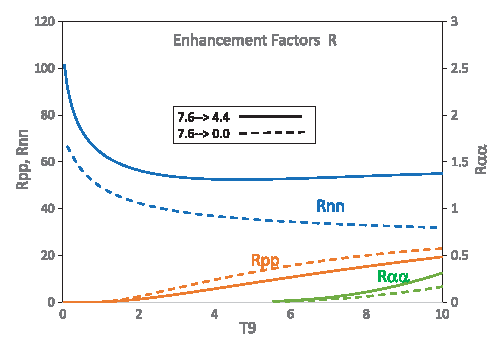
\includegraphics[clip, width=0.6\columnwidth]{eps/R_T.eps}
  \caption{}
  \label{fig::R}
\end{figure}

\section{最終的に狙うエネルギー領域}
$R$を計算するためには、実験によって断面積 ($\sigma_{nn'}$) のエネルギー分布が必要となる。
特に、天体中で${}^{12}\rm{C}$と散乱した後に中性子が持つエネルギー領域を狙う必要がある。
天体中の中性子の持つエネルギーはおよそ$k_{B}T$で表すことができる。
Beardら~\cite{hotdensemedium}が考えているような$T\sim10^{9}~\rm{K}$では、
中性子は$E_{n'}\sim100~\rm{keV}$で運動している。
このような中性子がHoyle状態の${}^{12}\rm{C}$と散乱すると、
散乱後の中性子は$E_{n}\sim8~\rm{MeV}$となる。
つまり、数〜十数$\rm{MeV}$のエネルギーを持つ中性子を用いて断面積のエネルギー分布が必要となる。
しかし、図\ref{fig::crosssection_pres}からも分かるように、数〜十数$\rm{MeV}$の領域のデータがない。
そのため、このエネルギー領域での ${}^{12}\rm{C}(n,n'){}^{12}\rm{C}^{Hoyle}$ の断面積の測定が必要である。
\begin{figure}
  \centering
  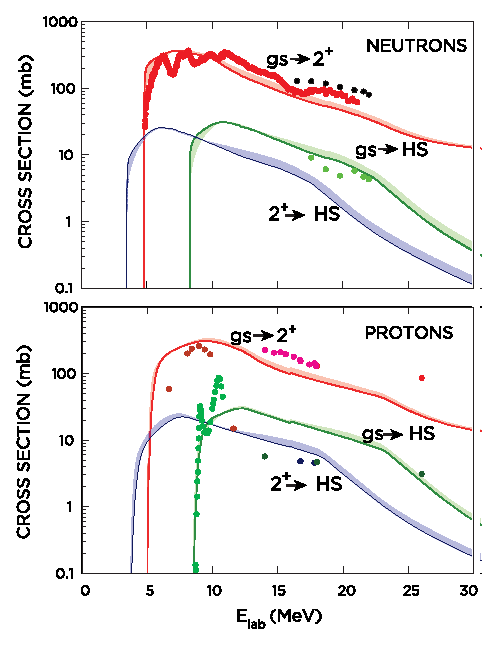
\includegraphics[clip,width=0.6\columnwidth]{eps/cross_section_p_and_n.eps}
  \caption{}
  \label{fig::crosssection_pres}
\end{figure}

本研究ではその第一歩として$E_{n} = 14.1~\rm{MeV}$の中性子を用いて断面積の測定を行う。
式 (\ref{eq::dt}) に示すDT反応で$14.1~\rm{MeV}$の単色中性子が生成可能である。
\begin{equation}
  \rm{d} + \rm{t} \rightarrow \alpha (3.5~\rm{MeV}) + \rm{n} (14.1~\rm{MeV})
  \label{eq::dt}
\end{equation}
このDT反応で生成される$14.1~\rm{MeV}$の中性子と炭素との反応は核融合炉の開発で重要である。
ITERなどの核融合炉ではDT反応を用いて質量エネルギーを取り出す。
$14.1~\rm{MeV}$の中性子は構造材の原子核と反応し損傷させるため、
構造材の中に多く含まれる炭素との反応が詳しく調べられてきた。
そのため、すでに$14.1~\rm{MeV}$の中性子と${}^{12}\rm{C}$との断面積のデータがあり、本研究での測定結果との比較が可能となる。
単色エネルギーの中性子を生成可能であること、他データと測定結果の比較が可能であることの2点より、
測定方法の検証として$14.1~\rm{MeV}$の中性子で断面積の測定を行う。

\section{先行研究}

\section{測定に用いる実験装置}
本研究では${}^{12}\rm{C}$のHoyle状態から崩壊して生成した3つの$\alpha$粒子を直接測定する。
$\alpha$粒子は数百$\rm{keV}$の運動エネルギーを持って生成する。
このようなエネルギーの$\alpha$粒子を効率よく検出するためには、
標的中で$\alpha$粒子が停止しないようにしなければならない。
例えば、$500~\rm{keV}$の$\alpha$粒子では炭素箔標的およそ$0.35~\rm{mg/cm^2}$で停止する。
また、すべて検出するためには大立体角を持つ検出器が必要となる。% alphaがどのくらいの立体角に産卵するかを言えると尚良
図\ref{fig::alpha_theta_dist}は$\alpha$粒子の角度分布を示す。
この図からもわかるようにほげほげ。
このような要求を満たす検出器としてMAIKo TPC ($\mu$-PIC based active target for inverse kinematics .
time projection chamber)~\cite{maiko, mupic}がある。
MAIKo TPC はTPC の検出ガスを散乱標的として用いる検出器であり、
低エネルギー粒子を大立体角で検出するために開発された。
\begin{figure}
  \centering
  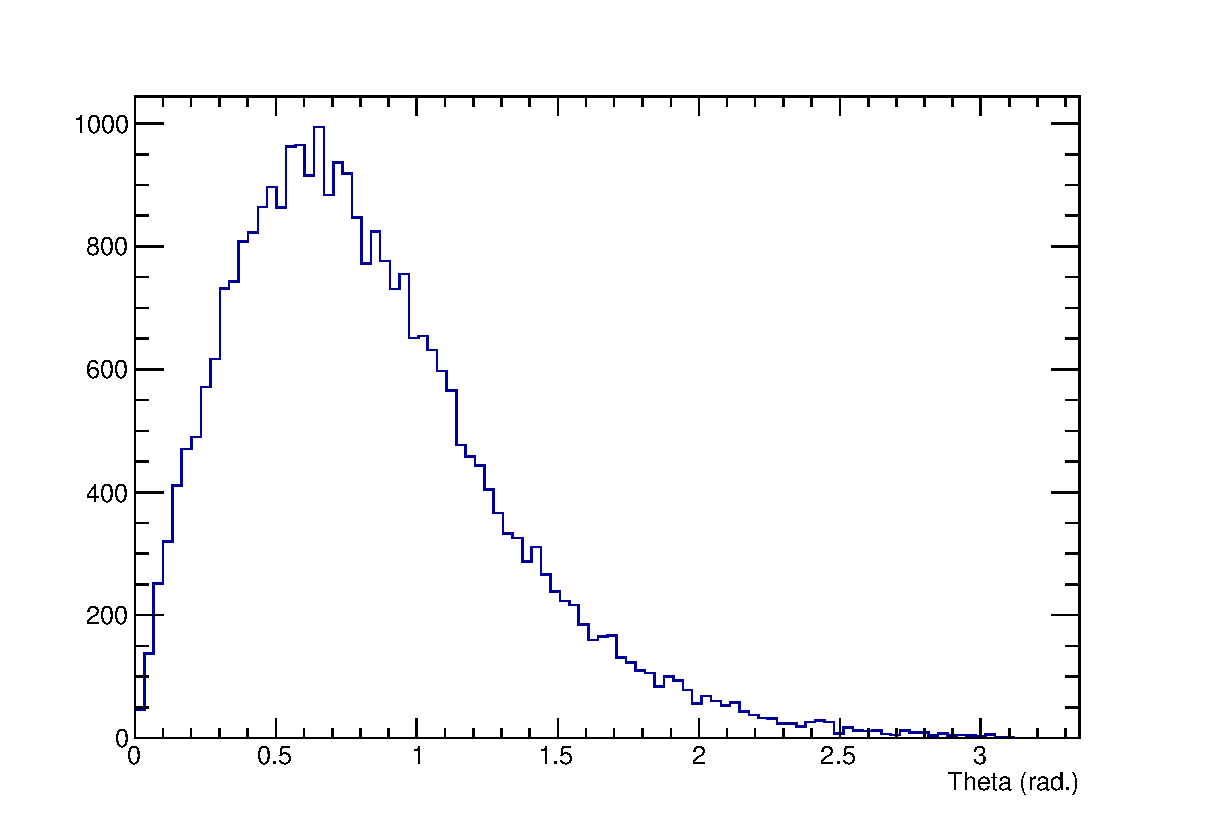
\includegraphics[clip, width=0.7\columnwidth]{eps/alpha_theta_dist.eps}
  \caption{}
  \label{fig::alpha_theta_dist}
\end{figure}

\section{本研究の目的}
\label{thiswork}
